\documentclass{article}
    % General document formatting
    \usepackage[margin=0.7in]{geometry}
    \usepackage[parfill]{parskip}
    \usepackage[utf8]{inputenc}
    \usepackage{amsmath}
    \usepackage{amssymb}
    \usepackage{tikz}
    \usepackage{fancyhdr}
    \usepackage{listings}

\pagestyle{fancy}
\fancyhf{}
\rhead{Edgar Jacob Rivera Rios - A01184125}

\begin{document}
\begin{titlepage}

    \newcommand{\HRule}{\rule{\linewidth}{0.5mm}} % Defines a new command for the horizontal lines, change thickness here

    \center % Center everything on the page

    %----------------------------------------------------------------------------------------
    %	HEADING SECTIONS
    %----------------------------------------------------------------------------------------

    \textsc{\LARGE Tecnológico de Monterrey}\\[1.5cm] % Name of your university/college
    \textsc{\Large Fundamentos de computación}\\[0.5cm] % Major heading such as course name
    %\textsc{\large Minor Heading}\\[0.5cm] % Minor heading such as course title

    %----------------------------------------------------------------------------------------
    %	TITLE SECTION
    %----------------------------------------------------------------------------------------

    \HRule \\[0.4cm]
    { \huge \bfseries Homework 5}\\[0.4cm] % Title of your document
    \HRule \\[1.5cm]

    %----------------------------------------------------------------------------------------
    %	AUTHOR SECTION
    %----------------------------------------------------------------------------------------

    \begin{minipage}{0.4\textwidth}
    \begin{flushleft} \large
    \emph{Student:}\\
    Jacob \textsc{Rivera} % Your name
    \end{flushleft}
    \end{minipage}
    ~
    \begin{minipage}{0.4\textwidth}
    \begin{flushright} \large
    \emph{Professor:} \\
    Dr. Hugo \textsc{Terashima} % Supervisor's Name
    \end{flushright}
    \end{minipage}\\[2cm]

    % If you don't want a supervisor, uncomment the two lines below and remove the section above
    %\Large \emph{Author:}\\
    %John \textsc{Smith}\\[3cm] % Your name

    %----------------------------------------------------------------------------------------
    %	DATE SECTION
    %----------------------------------------------------------------------------------------

    {\large \today}\\[2cm] % Date, change the \today to a set date if you want to be precise

    %----------------------------------------------------------------------------------------
    %	LOGO SECTION
    %----------------------------------------------------------------------------------------

    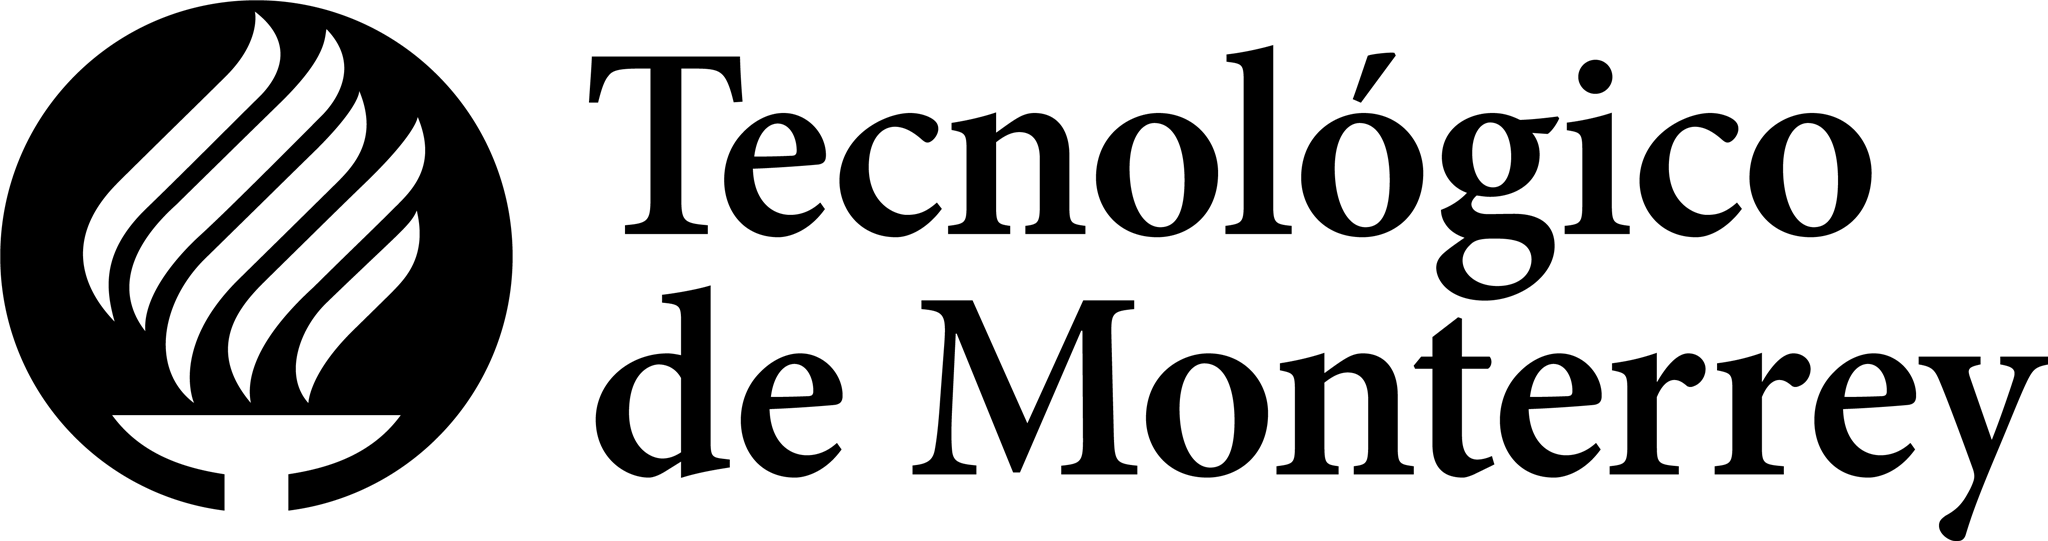
\includegraphics[width=0.4\textwidth,height=\textheight,keepaspectratio]{logo-tec-negro.png} % Include a department/university logo - this will require the graphicx package

    %----------------------------------------------------------------------------------------

    \vfill % Fill the rest of the page with whitespace

\end{titlepage}


\section{Problems}
Solve the following problems:
\begin{enumerate}
    \item Implement algorithms quicksort, mergesort and heapsort in any programming language, and investigate their performance in arrays of size $10^2$, $10^3$, $10^4$, $10^5$ and $10^6$. For each of those sizes, consider files of  randomly-generated  integers,  files  with  integers  already  sorted  in  ascending  order,  and  files  with integers already sorted in descending order. Hand in a report with your investigation containing the analysis, discussion of results and the conclusions.

    \begin{center}
        \begin{tabular}{|c|c|c|c|c|c|c|c|c|c|}
            \hline
            &QS &QS &QS &Merge  &Merge &Merge &Heap &Heap &Heap\\
            &Random &Ordered &Reverse &Random &Ordered &Reverse &Random &Ordered &Reverse\\
            \hline
            $10^2$& $1.75e^{-5}$s & $1.29e^{-5}$s & $1.38e^{-5}$s & & & & & & \\
            $10^3$& $1.98e^{-4}$s & $1.52e^{-4}$s & $1.58e^{-4}$s & & & & & & \\
            $10^4$& $2.22e^{-3}$s & $1.6e^{-3}$s & $1.67e^{-3}$s & & & & & & \\
            $10^5$& $2.42e^{-2}$s & $1.67e^{-2}$s & $1.75e^{-2}$s & & & & & & \\
            $10^6$& $0.257$s& $0.178$s & $0.184$s & & & & & & \\
            \hline
        \end{tabular}
    \end{center}

    \item Consider the 3-ary heap, similar to the binary heap, except that a no-leaf node has 3 siblings
    \begin{enumerate}
        \item How would you represent a 3-ary heap in an array?
        \item What is the height of a 3-ary heap with $n$ elements, in terms of $d = 3$ and $n$?
        \item For an element in position $i$ in the heap, determine the position of its parent and siblings.
        \item In general terms, determine the complexity of a heap algorithm with these features.
    \end{enumerate}

    \item Show how a set of $n$ positive integers between 1 and $n^2$ can be sorted in linear time
    \item Describe and algorithm that makes 42 comparisons for sorting 15 elements in the worst case (Donald Knuth, The Art of Computer Programming, Vol. 3). Show how the algorithm works using an example.
\end{enumerate}
\end{document}